\csname documentclass\endcsname[../main.tex]{subfiles}
\begin{document}
\chapter{Background and Related Work}

\section{CBM}\label{background:cbm}

Concept Bottleneck Models (CBMs), initially proposed by Koh et al.~\cite{cbm}, are a class of models
that consist of a model $g$ that learns a mapping from
input $\mathbf{x}$ to a concept vector $\mathbf{c} = g(\mathbf{x})$, 
where $\mathbf{c}$ is a multi-hot encoding of the concepts present in the input,
and a model $f$
that learns a mapping from such concepts vector $c$
to the output label $\mathbf{y} = f(\mathbf{c})$, as shown in Figure~\ref{fig:cbm}.
These types of model can be created by simply adding a new layer in traditional models
with the same number of neurons as the number of concepts, where this layer
is referred to as the "CBM Bottleneck". 
Henceforth $g$ is referred to as the ``concept predictor $\mathbf{x} \to \mathbf{c}$ model'' and $f$ as the
``label $\mathbf{c} \to \mathbf{y}$ predictor model''.
 Training such a model requires a
dataset of inputs $\mathbf{x}$ annotated with the corresponding 
concepts $\mathbf{c}$ and labels $\mathbf{y}$. 

\begin{figure}[!h]
    \centering
    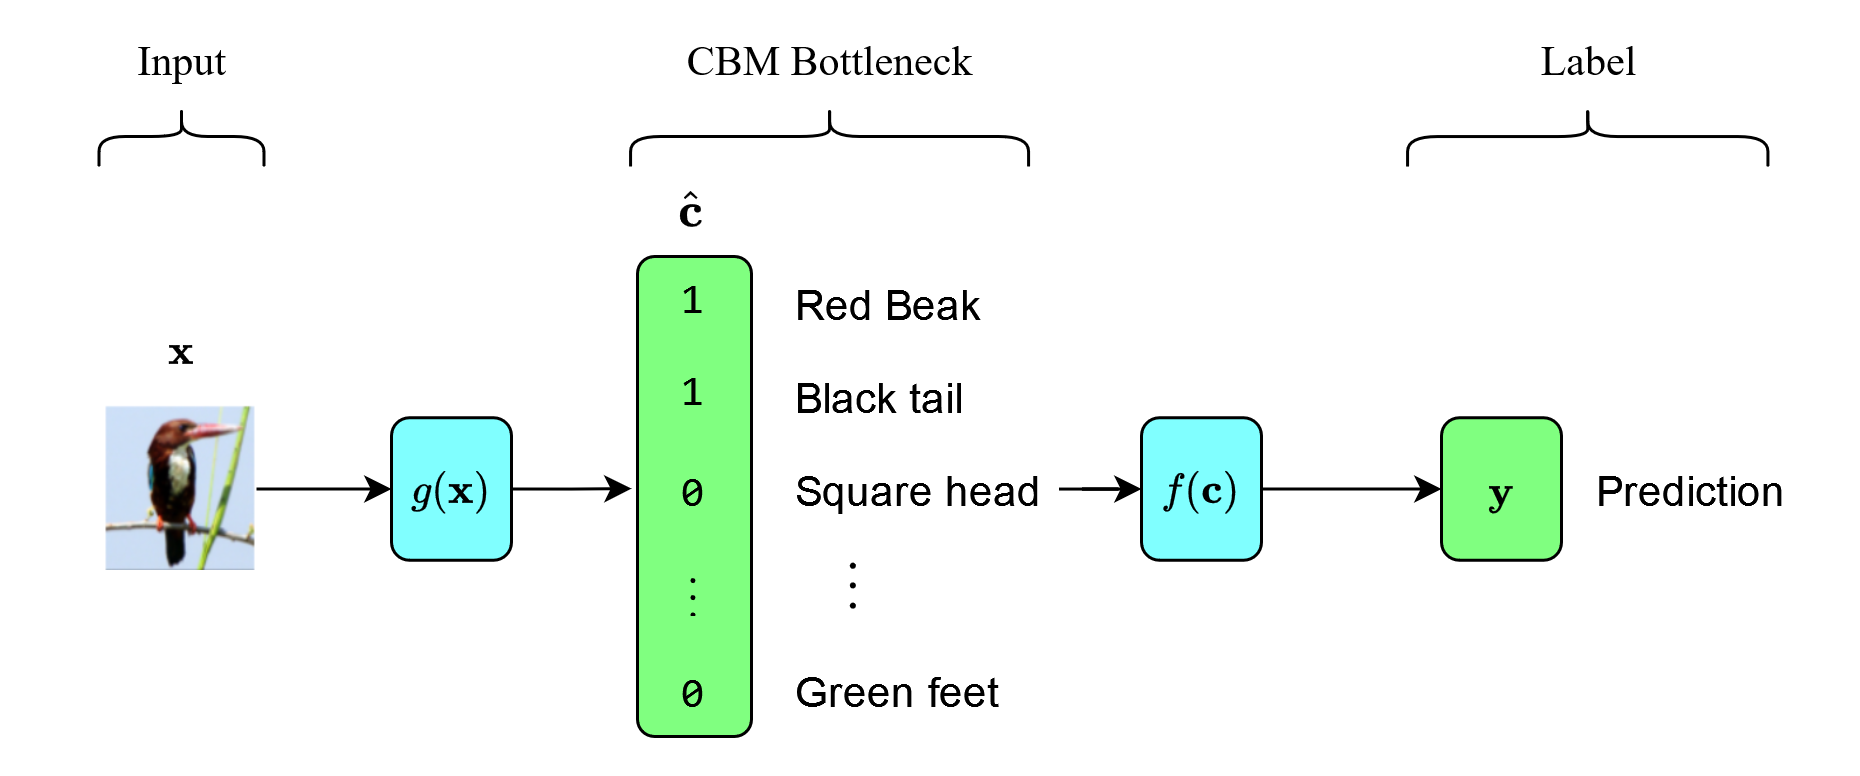
\includegraphics[width=\textwidth]{figs/background/cbm.png}
    \caption{The CBM Architecture~\cite{cbm}.}
    \label{fig:cbm}
\end{figure}

CBMs allow for interventions, which are using experts to correct the intermediate concepts
predicted by the $\mathbf{x} \to \mathbf{c}$ model to improve the performance of the $\mathbf{c} \to \mathbf{y}$ model,
which is illustrated in Figure~\ref{fig:cbm-interventions}

\begin{figure}[!h]
    \centering
    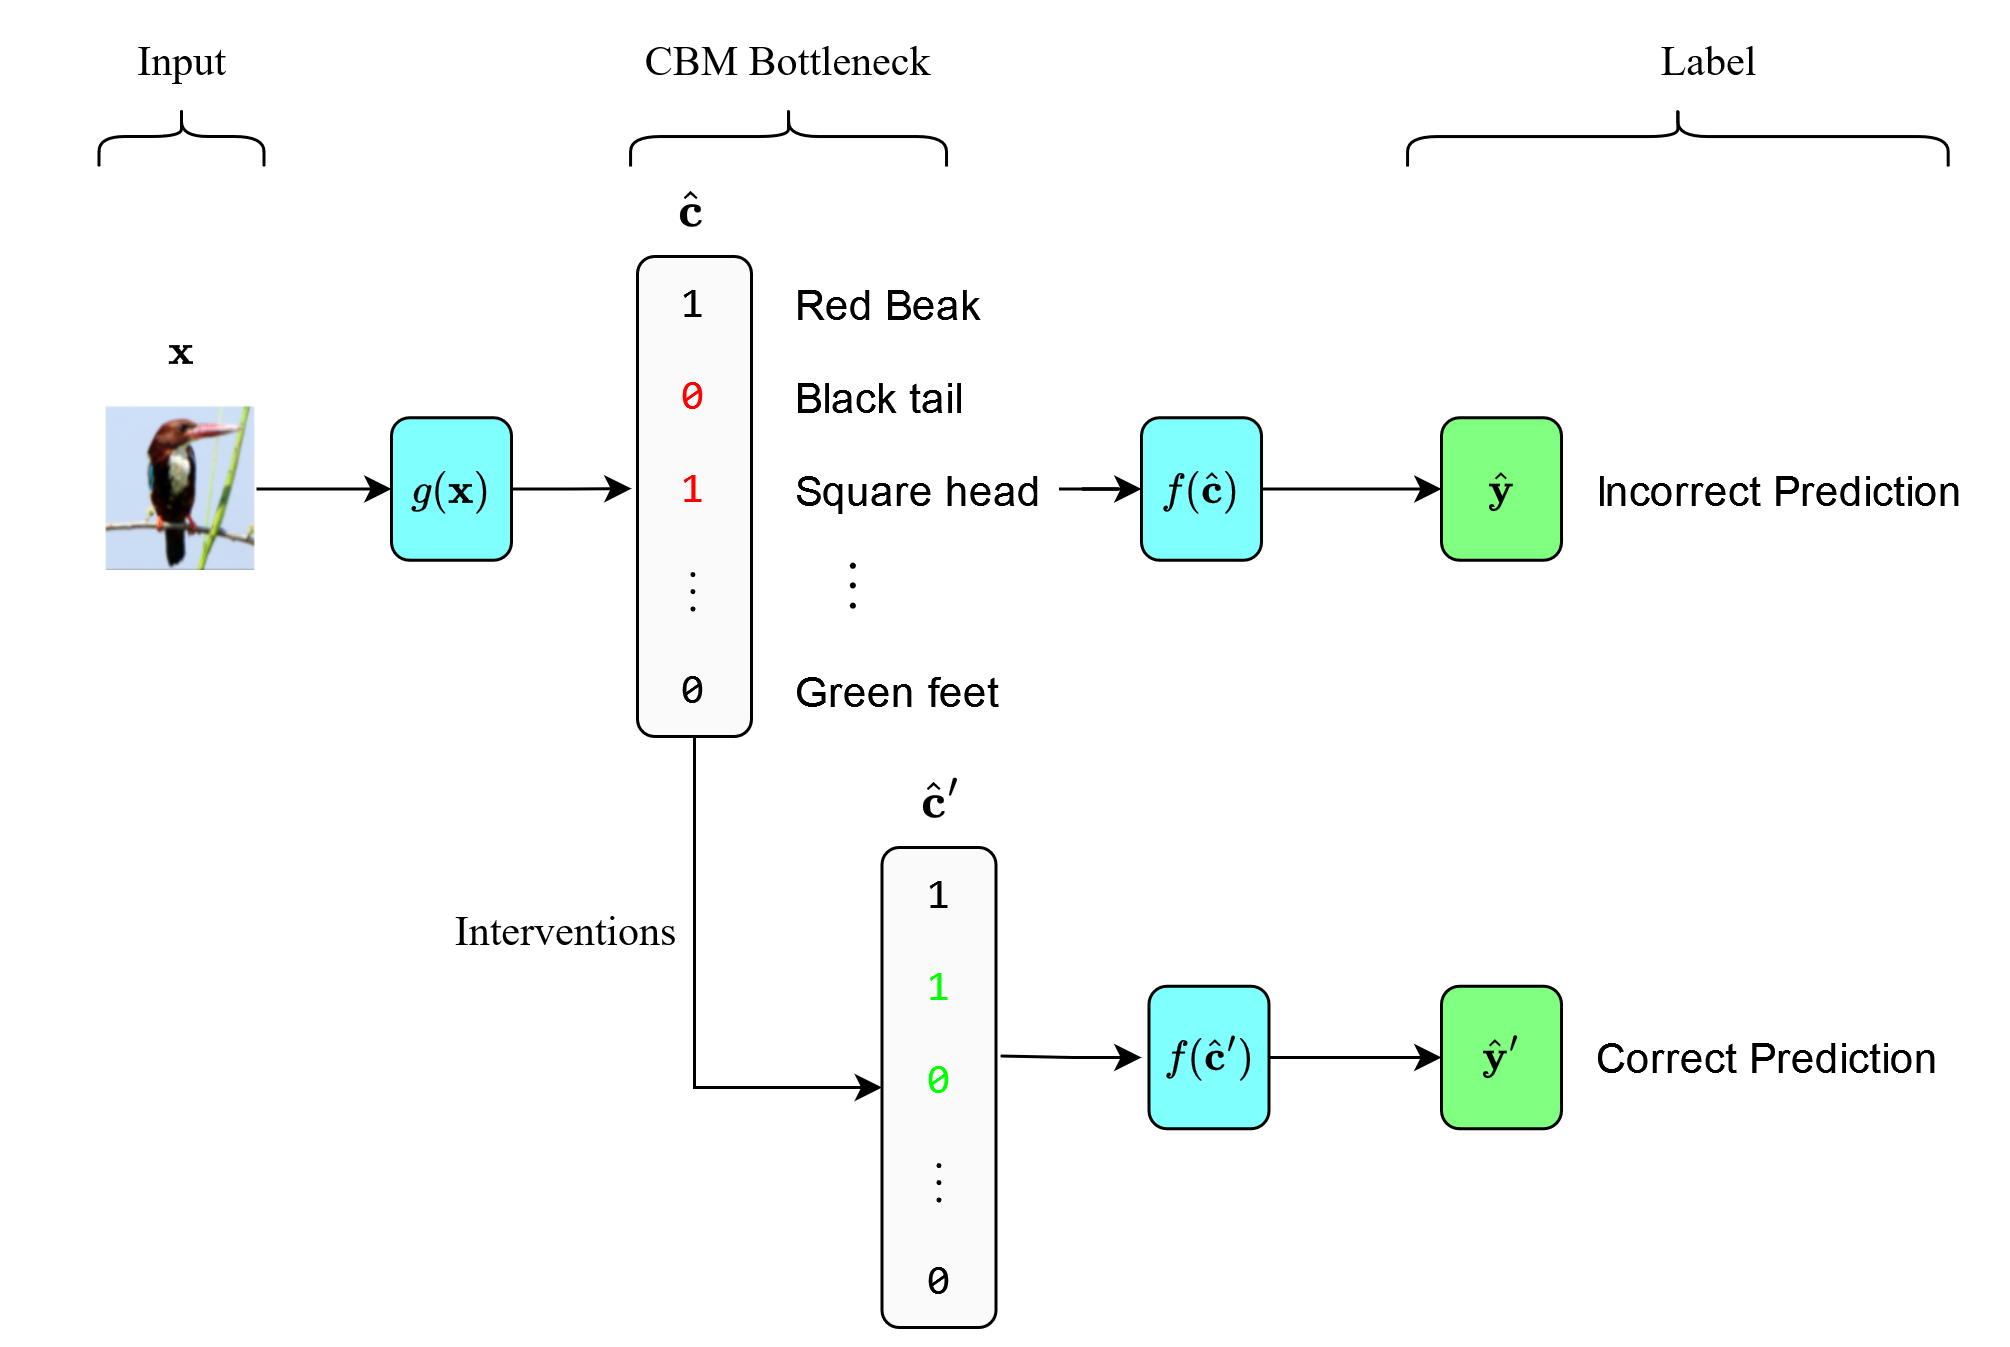
\includegraphics[width=\textwidth]{figs/background/cbm_interventions.png}
    \caption{An illustration of intervening on the concepts predicted by a CBM.}
    \label{fig:cbm-interventions}
\end{figure}

\subsection{Training CBMs}

There are several different ways to train a CBM. 
If we let the concept loss $L_{\text{concept}}$ be a loss
 function that measures
the discrepancy between the predicted concepts $\hat{\mathbf{c}}$
and the actual concepts $\mathbf{c}$, and similarly the 
label loss $L_{\text{label}}$ measuring the discrepancy
between the predicted concepts $\hat{\mathbf{y}}$
and the actual concept $\mathbf{y}$,
both losses as illustrated in Figure~\ref{fig:cbm}.
There are the following ways
to train a CBM as proposed in~\cite{cbm}.

\begin{enumerate}
    \item Independent: Training the two models independently by minimizing
    $L_{\text{concept}}(g(\mathbf{x}), \mathbf{c})$ and $L_{\text{label}}(f(\mathbf{c}), \mathbf{y})$ independently.
    \item Sequential: Training the models one by one, first learning
    $\hat{g}$ by minimizing 
    
    $L_{\text{concept}}(g(\mathbf{x}), \mathbf{c})$,
    then learning $f$ by minimizing $L_{\text{label}}(f(\mathbf{\hat{g}(\mathbf{x})}), \mathbf{y})$
    \item Joint: The model is trained via a weighted sum of the losses given by \\ 
    $\lambda_{\text{concept}} L_{\text{concept}}(g(\mathbf{x}), \mathbf{c}) + \lambda_{\text{label}} L_{\text{label}}(f(g(\mathbf{x})), \mathbf{y})$ \\
    such that both losses are minimised simultaneously.
\end{enumerate}

It has been shown experimentally that while the joint models perform the best
without interventions, followed by the sequential model, and the independent model
performs the worst. This is because the sequential model allows the $\mathbf{c} \to \mathbf{y}$ 
model to learn a mapping from the concepts produced by the $\mathbf{x} \to \mathbf{c}$ model to
label $\mathbf{y}$, where the concepts produced by the $\mathbf{x} \to \mathbf{c}$ model is often different
from the true concepts, an underlying requirement for the independent model to perform well. Additionally,
the joint model allows the $\mathbf{x} \to \mathbf{c}$ model to simultaneously learn to output a representation
of concepts that allow for best performance of the $\mathbf{c} \to \mathbf{y}$ model~\cite{cbm}.

When comparing performance under interventions,
independent models outperform the two models.
They are more sensitive to interventions and each successive intervention step
leads to a bigger increase in performance compared to the other two,
with better performances after the same number of interventions.
The reason behind this
is that the independent model learns a mapping from the true concepts to the label,
whereas the other two learn a mapping from the predicted concepts to the label. Each intervention
modifies the predicted concepts to be closer to the true concepts, which is what the 
$\mathbf{c} \to \mathbf{y}$ independent model is trained to do~\cite{cbm}.

\section{CEM}\label{background:cem}

While CBMs proved to be useful in achieving machine learning models with high
interpretability, they do not perform as well as traditional models that learn a direct
mapping from input to labels. This is because the CBM label
prediction model relies only on a set of human-interpretable concepts, which limits
the performance of the model as traditional models can extract
information outside of these concepts that are potentially not human-interpretable~\cite{cem}. 
This is even more apparent
if the dataset does not contain a complete set of concepts that cover all
features present in the input, which is very common in real-life scenarios.
As such, there is a trade-off between performance and interpretability, where researchers
have developed methods such as extending the CBM bottleneck with a set of unsupervised neurons
to increase accuracy at a cost of decreasing interpretability~\cite{cbm-hybrid}.

To overcome this trade-off, Concept Embedding Models (CEMs) were proposed by Zarlenga et al.~\cite{cem},
these are CBMs that further add an additional layer of learnable embeddings before
the original bottleneck, learning two embedding vectors for each concept: one for
when the concept is and is not present. The architecture of CEMs is shown in Figure~\ref{fig:cem}.
An intermediate scoring function $\phi_i$ is learnt for each concept $i$, 
and the embedding assigned to the bottleneck is an interpolation of the two embeddings
based on the scoring function predicting the possibility of the concept to be present.

This architecture also allows for interventions during run-time. By simply modifying the
output of the scoring function to be that of the true concept, the bottleneck 
can be modified similarly to CBMs and improve the performance of the model. Additionally
to increase the performance of CEMs, the authors utilised observations mentioned in
Section~\ref{background:cbm}, where models trained on the true concepts are more sensitive to 
interventions. They proposed RandInt, a method to randomly intervene
during training with $\lambda_{\text{int}} = 0.25$ probability of intervening
on a concept. They show that this effectively boosts the performance of the model 
under interventions during test time without notable effects to the performance 
without interventions~\cite{cem}.

CEMs successfully solves the trade-off problem between performance and interpretability,
allowing for similar performance to traditional models while maintaining the
interpretability, along with high concept accuracy. This is because the embedding structure
for CEMs allow for encoding of more information
in the concept representations and is more machine-interpretable, where
the additional information in the bottleneck
 compared to scalar representations in CBMs
lead to a better performing label predictor model. Additionally CEMs are still trained 
on the same set of human-interpretable concepts as CBM via a similar concept loss, which leads to
high interpretability and good intervention performance. It has been shown experimentally
that CEMs are able to provide better performance for concept-incomplete dataset tasks (where
the concepts do not cover all features present in input), and these learnt concept
embedding representations effectively represent the true concepts measured by an alignment score~\cite{cem}.


\section{IntCEM} % 500

Building on top of CEMs, Zarlenga et al.~\cite{intcem} introduced 
Intervention-aware CEM (IntCEM), which are CEMs that are augmented
with a learnable concept intervention policy model. IntCEMs' novelty
lies in framing the problem of training a CEM and finding
an intervention policy as a joint optimization problem by augmenting
existing CEMs with a trainable intervention policy model $\psi$. 
This approach offers significant improvements in performance after 
interventions while maintaining similar performance without 
interventions. 
IntCEM achieves this because the intervention policy model
learn a good intervention policy specific to the CEM, 
and the CEM also learns to be more sensitive to interventions
by the model, through the introduction of an intervention loss 
$L_{\text{int}}$ and task loss $L_{\text{task}}$ for 
the intervened concepts.

During training, $\psi$ first samples intervention
logits for the next concept to intervene on, then 
a Cross Entropys loss $L_{\text{int}}$ is used to
compute the discrepancy with the output of a greedy 
optimal policy, found by searching over all concept to
yield the concept that leads to the highest increase
in model performance when intervened. This is a Behavioural
Cloning~\cite{} approach where $\psi$ learns to clone the behaviour of
a greedy optimal policy.

As mentioned in Section~\ref{background:cbm}, training using
true concept labels increases the model's sensitivity
to interventions, leading to better intervention performance.
IntCEM incorporates this idea by computing task loss
using the intervened concepts by $\psi$ during training.
Not only does this increase the model's sensitivity to interventions,
it specifically increases the model's sensitivity to interventions
sampled by $\psi$ to further improve its intervention performance.

\section{RL}\label{background:rl} % 500
Reinforcement Learning is a machine learning subfield that 
focuses on training agents to make sequential decisions in an environment.
Contrary to supervised learning
where the goal is to minimize the discrepancy between predicted outputs and true outputs,
the goal of Reinforcement Learning is to maximize the cumulative rewards received by the agent
by taking actions over time. The agent has access to observations which reflect the current state
 of the environment and can take actions to progress to different states until 

 The PPO algorithm is a policy gradient method that 
combines the strengths of traditional policy-based approaches
and value-based approaches~\cite{deep-q-learning, deep-q-learning-2}

and 
is one of the most popular Reinforcement Learning algorithms for learning
an optimal policy due to its robustness.
 
\section{Flow Models}\label{background:flow}
Flow models model probability distributions by leveraging the change of variable property~\cite{normalizing-flows}.
Given an input distribution $x \sim p_X(\mathbf{x})$, the change of variable property allows us to define
deterministic invertible transformations $f: \mathbf{x} \to \mathbf{z}$, such that 
$\mathbf{z} = f(\mathbf{x})$ where there exists a simple invertible function
$f^{-1}$ such that $\mathbf{z} = f^{-1}(f(z)) \forall z$. 



Flow models define transformations
using ML models with this property with learnable parameters

Each of these transformations give a normalized
density, and they can be composed to create more complex invertible distributions.
This property allows us to define normalizing flow models which learn a series of transformations
that use a simple latent distribution to model a complex distribution, such as 
the distribution of concepts within a dataset for CEMs.

\section{Related Work}


\subsection{CooP}

\subsection{Active Feature Acquisition}


\end{document}